% =========================================================================
%  Digital Religions @ UZH — 25-minute talk
%  Transformer-Based Cross-Lingual Approaches to Religious Hate Speech
%  Zhidian Huang · based on MA thesis (UZH)
%
%  Compile with:  xelatex slides.tex   (twice)
%  xeCJK is used so that Chinese / Japanese examples render correctly.
%  If Noto CJK is not installed, replace the \setCJKmainfont line with
%  another CJK font available on your system (e.g. "Source Han Serif SC").
% =========================================================================
\documentclass[aspectratio=169,10pt]{beamer}

% ---- Theme & look ---------------------------------------------------------
\usetheme{default}
\usecolortheme{default}
\setbeamertemplate{navigation symbols}{}
\setbeamertemplate{footline}[frame number]
\setbeamertemplate{itemize items}[circle]
\setbeamertemplate{itemize subitem}[triangle]

\definecolor{uzhblue}{RGB}{0,40,85}
\definecolor{uzhaccent}{RGB}{160,30,50}
\definecolor{mutedgray}{RGB}{90,90,90}
\definecolor{softbg}{RGB}{245,245,245}

\setbeamercolor{title}{fg=uzhblue}
\setbeamercolor{frametitle}{fg=uzhblue}
\setbeamercolor{structure}{fg=uzhblue}
\setbeamercolor{alerted text}{fg=uzhaccent}
\setbeamercolor{block title}{bg=uzhblue,fg=white}
\setbeamercolor{block body}{bg=softbg,fg=black}

\setbeamerfont{frametitle}{series=\bfseries,size=\large}
\setbeamerfont{title}{series=\bfseries,size=\Large}

% ---- Packages -------------------------------------------------------------
\usepackage{fontspec}
% xeCJK is needed so the Chinese / Japanese examples in the slides render.
% It is loaded only if available; otherwise the CJK characters simply render
% in the default font (which may fall back to tofu on some machines).
\IfFileExists{ctexhook.sty}{%
  \usepackage{xeCJK}%
  \IfFontExistsTF{Noto Serif CJK SC}{\setCJKmainfont{Noto Serif CJK SC}}{%
    \IfFontExistsTF{Source Han Serif SC}{\setCJKmainfont{Source Han Serif SC}}{}}%
  \IfFontExistsTF{Noto Sans CJK SC}{\setCJKsansfont{Noto Sans CJK SC}}{}%
}{}

\usepackage{graphicx}
\graphicspath{{images/}}
\usepackage{tikz}
\usetikzlibrary{positioning,arrows.meta,shapes.geometric,fit,backgrounds,calc}
\usepackage{booktabs}
\usepackage{array}
\usepackage{tabularx}
\usepackage{xcolor}
\usepackage{hyperref}
\usepackage{amsmath}
\usepackage{adjustbox}

% ---- Handy macros ---------------------------------------------------------
\newcommand{\emphc}[1]{\textcolor{uzhaccent}{\textbf{#1}}}
\newcommand{\keyword}[1]{\textcolor{uzhblue}{\textbf{#1}}}
\newcommand{\takeaway}[1]{%
  \vspace{0.3em}
  \begin{block}{Takeaway}#1\end{block}}

% ---- Title ----------------------------------------------------------------
\title[Cross-Lingual Religious Hate Speech]{%
  From Detection to Interpretation\\
  \large Transformer-Based Cross-Lingual Approaches to Religious Hate Speech}
\subtitle{A \emph{who--how--why} framework for Digital Religion research\\
  Case: Anti-Christian discourse in Chinese, Japanese, and English}
\author{Zhidian Huang}
\institute{University of Zurich · Department of Computational Linguistics}
\date{Digital Religions Conference, UZH\\ \today}

% =========================================================================
\begin{document}
% =========================================================================

% ---- Slide 1: Title -------------------------------------------------------
\begin{frame}[plain]
  \titlepage
  \vspace{-0.5em}
  \begin{center}\small
  \textit{``How computational methods can reveal cross-cultural\\
  structures of religious hostility in digital spaces.''}
  \end{center}
\end{frame}

% ---- Slide 2: Why this matters for this audience --------------------------
\begin{frame}{Why this talk belongs at Digital Religions}
  \begin{columns}[T,onlytextwidth]
    \begin{column}{0.55\textwidth}
    \small
    Digital-religion scholarship asks \keyword{how religion is contested
    online}. That question is increasingly answered at a \keyword{scale}
    that manual reading alone cannot cover.
    \vspace{0.6em}

    Most NLP work, by contrast, still asks only:\\
    \centerline{\textit{``is this post hate speech — yes / no?''}}
    \vspace{0.6em}

    My question is different:
    \begin{itemize}
      \item \emphc{What kinds of anti-religious narratives emerge
      \emph{across cultures}}, once we stop forcing a binary label?
    \end{itemize}
    \vspace{0.5em}
    \textit{Bridge.} This re-purposes AI as an \keyword{interpretive tool}
    for religion research — letting the data itself reveal the
    \keyword{forms} that religious hostility takes online.
    \end{column}
    \begin{column}{0.42\textwidth}
    \centering\footnotesize
    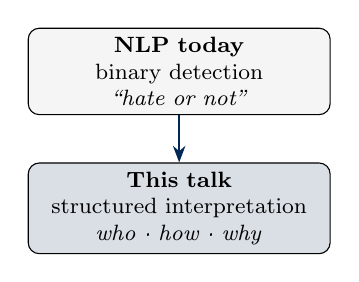
\begin{tikzpicture}[every node/.style={font=\footnotesize}]
      \node[draw,rounded corners,fill=softbg,text width=3.6cm,align=center,minimum height=1cm] (a)
        {\textbf{NLP today}\\ binary detection\\ \textit{``hate or not''}};
      \node[draw,rounded corners,fill=uzhblue!15,text width=3.6cm,align=center,minimum height=1cm,below=0.6cm of a] (b)
        {\textbf{This talk}\\ structured interpretation\\ \textit{who · how · why}};
      \draw[-{Stealth[length=6pt]},thick,uzhblue] (a) -- (b);
    \end{tikzpicture}
    \end{column}
  \end{columns}
\end{frame}

% ---- Slide 3: Research gap ------------------------------------------------
\begin{frame}{A three-fold research gap}
  \begin{enumerate}
    \item \keyword{Religion in NLP} $\approx$ Islamophobia + antisemitism.\\
      \textit{Anti-Christian hostility is comparatively under-studied.}
    \vspace{0.4em}
    \item \keyword{Languages}. Chinese and Japanese are rarely part of
      cross-lingual benchmarks; zero-subject grammar further breaks
      standard parsers.
    \vspace{0.4em}
    \item \keyword{Task formulation}. Binary classification cannot tell us
      \emph{who} is targeted, \emph{how} the attack is framed, or
      \emph{why} it is morally persuasive in a given community.
  \end{enumerate}
  \vspace{0.6em}
  \takeaway{We need an \emph{interpretable, cross-lingual} analytical
  framework — not a better hate-speech detector.}
\end{frame}

% ---- Slide 3.5: Why anti-Christian? ---------------------------------------
\begin{frame}{Why use anti-Christian discourse as the probe?}
  Christianity is analytically unusual because its social position
  \keyword{varies sharply} across the three communities we study:
  \vspace{0.4em}
  \begin{itemize}
    \item \keyword{English} — historically \emph{dominant}, often critiqued
      from \textbf{within} a shared normative framework.
    \item \keyword{Chinese} — a \emph{minority} faith frequently framed
      through \textbf{foreign influence}, missionary history, and state
      regulation.
    \item \keyword{Japanese} — a \emph{small} minority, but politically
      salient after the Abe/Unification-Church scandal of 2022.
  \end{itemize}
  \vspace{0.6em}
  \textit{The same target, three distinct social positions:}
  a natural laboratory for asking whether hate discourse is
  \emphc{universal} or \emphc{context-dependent}.
  \vspace{0.4em}\\
  \footnotesize The goal is \emph{not} to privilege one religion, but to
  use Christianity as a \keyword{comparative probe}.
\end{frame}

% ---- Slide 4: Research questions -----------------------------------------
\begin{frame}{Three linked questions}
  \begin{columns}[T,onlytextwidth]
    \begin{column}{0.5\textwidth}
    \small
    \begin{itemize}
      \item \textbf{RQ1 — \emphc{Who}} is targeted? \\
        {\footnotesize Institutions, clergy, believers, public figures?}
      \item \textbf{RQ2 — \emphc{How}} is hostility expressed? \\
        {\footnotesize Which rhetorical / thematic frames recur?}
      \item \textbf{RQ3 — \emphc{Why}} does it persuade locally? \\
        {\footnotesize Which moral vocabularies carry the attack?}
    \end{itemize}
    \vspace{0.6em}

    Together they form a reusable
    \textcolor{uzhblue}{\textbf{\textit{who--how--why} framework}}
    for digital-religion analysis.
    \end{column}
    \begin{column}{0.48\textwidth}
    \centering
    \vspace{0.3em}
    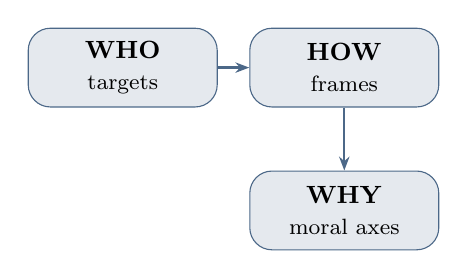
\begin{tikzpicture}[
      pill/.style={rectangle, rounded corners=8pt, draw=uzhblue!70,
                   fill=uzhblue!10, minimum width=2.4cm, minimum height=1cm,
                   align=center, font=\small},
      arr/.style={-{Stealth[length=5pt]}, thick, uzhblue!70}]
      \node[pill] (who)  {\textbf{WHO}\\\footnotesize targets};
      \node[pill, right=0.4cm of who] (how) {\textbf{HOW}\\\footnotesize frames};
      \node[pill, below=0.8cm of how] (why) {\textbf{WHY}\\\footnotesize moral axes};
      \draw[arr] (who) -- (how);
      \draw[arr] (how) -- (why);
    \end{tikzpicture}\\[0.4em]
    \footnotesize\itshape
    \textcolor{uzhblue}{a reusable structured-interpretation framework}
    \end{column}
  \end{columns}
\end{frame}

% ---- Slide 5: Data --------------------------------------------------------
\begin{frame}{A trilingual corpus of 63{,}265 texts}
  \small
  \begin{tabularx}{\textwidth}{l X r}
    \toprule
    \textbf{Language} & \textbf{Sources} & \textbf{Texts} \\
    \midrule
    English  & Existing hate-speech datasets, curated forum threads &
      \textasciitilde 21k \\
    Chinese  & Tieba + web corpora, custom annotation &
      \textasciitilde 18k \\
    Japanese & 5ch + Common Crawl, custom annotation &
      \textasciitilde 24k \\
    \bottomrule
  \end{tabularx}
  \vspace{0.5em}
  \begin{itemize}
    \item For low-resource settings, we use \keyword{LLM-assisted
      back-translation augmentation} rather than translating from English
      (which would import English framings).
    \item Annotation is \emphc{structured}: target, attack frame, and
      moral axis — not only ``hate / not-hate''.
  \end{itemize}
  \takeaway{A balanced trilingual resource lets us compare
  \emph{framings} on equal footing — and is released open-source:
  \href{https://github.com/notsofun/Master_Thesis}{\texttt{github.com/notsofun/Master\_Thesis}}.}
\end{frame}

% ---- Slide 6: Method (overview) ------------------------------------------
\begin{frame}{Pipeline: from raw text to structured meaning}
  \small
  \centering
  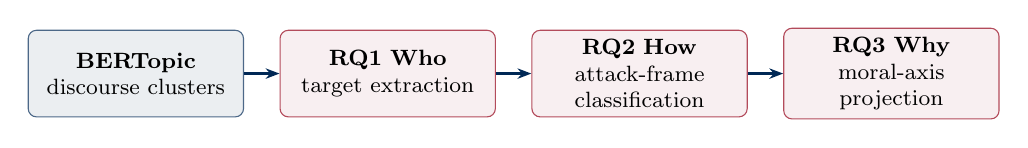
\begin{tikzpicture}[
    node distance=0.5cm and 0.45cm,
    box/.style  ={rectangle, rounded corners=3pt, draw=uzhblue!70, fill=uzhblue!8,
                  text width=2.5cm, align=center, minimum height=1.1cm, font=\footnotesize},
    rqbox/.style={rectangle, rounded corners=3pt, draw=uzhaccent!80, fill=uzhaccent!7,
                  text width=2.5cm, align=center, minimum height=1.1cm, font=\footnotesize},
    arr/.style  ={-{Stealth[length=5pt]}, thick, uzhblue}]
    \node[box]                  (bt) {\textbf{BERTopic}\\ discourse clusters};
    \node[rqbox, right=of bt]   (r1) {\textbf{RQ1 Who}\\ target extraction};
    \node[rqbox, right=of r1]   (r2) {\textbf{RQ2 How}\\ attack-frame classification};
    \node[rqbox, right=of r2]   (r3) {\textbf{RQ3 Why}\\ moral-axis projection};
    \draw[arr] (bt) -- (r1);
    \draw[arr] (r1) -- (r2);
    \draw[arr] (r2) -- (r3);
  \end{tikzpicture}
  \vspace{0.4em}
  \begin{columns}[T,onlytextwidth]
    \begin{column}{0.54\textwidth}\footnotesize
      \textbf{Design principle.}
      \begin{itemize}
        \item \emphc{Induce} structure from the corpus, don't impose an
          English-trained taxonomy.
        \item \emphc{Modular} stages — each can be inspected, challenged,
          or replaced by a scholar.
        \item \emphc{Interpretable outputs} — a target label, a frame
          label, a moral vector.
      \end{itemize}
    \end{column}
    \begin{column}{0.44\textwidth}\footnotesize
      \textbf{Why not supervised end-to-end?}
      \vspace{0.2em}\\
      Pure supervised classifiers reproduce the labels we already have
      (mostly English, mostly Islamophobia / antisemitism). Unsupervised
      clustering lets new regions of the discourse \emph{surface}
      themselves — including the Unification-Church cluster that nobody
      pre-labelled.
    \end{column}
  \end{columns}
\end{frame}

% ---- Slide 6b: Method (short technical zoom) -----------------------------
\begin{frame}{One technical slide — how the pieces fit}
  \small
  \begin{columns}[T,onlytextwidth]
    \begin{column}{0.55\textwidth}
    \textbf{Shared backbone.}\\
    Multilingual E5-large (1024-d) encodes every sentence. A small
    mean-centring step per language aligns the three sub-spaces.
    \vspace{0.4em}\\
    \textbf{BERTopic} (UMAP + HDBSCAN) then clusters the aligned
    embeddings into \keyword{47 discourse topics} — monolingual topics
    live next to genuinely cross-lingual ones.
    \vspace{0.4em}\\
    \textbf{For RQ2} we add a predicate-window extractor to cope with
    Chinese and Japanese zero-subject sentences, then an LLM classifier
    into \keyword{10 author-constructed attack frames}.
    \vspace{0.4em}\\
    \textbf{For RQ3} we build seven \keyword{moral axes}
    (5 MFT + 2 intergroup-threat) as centroid differences of dictionary
    words, and project every document onto them:
    \[
      \mathrm{Bias}(d,k)\;=\;\cos\!\bigl(\text{E5}(d),\,\mathbf{a}_k\bigr).
    \]
    \end{column}
    \begin{column}{0.43\textwidth}\footnotesize
    \textbf{Axis = virtue centroid $-$ vice centroid}
    \vspace{0.3em}
    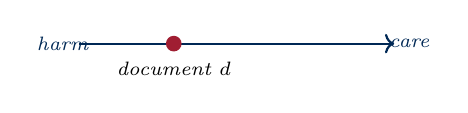
\begin{tikzpicture}[every node/.style={font=\scriptsize}]
      \draw[->,thick,uzhblue] (-2.0,0) -- (2.0,0);
      \node[uzhblue] at (-2.2,0) {\textit{harm}};
      \node[uzhblue] at ( 2.2,0) {\textit{care}};
      \node[circle,fill=uzhaccent,inner sep=2pt,label=below:\textit{document $d$}] at (-0.8,0) {};
    \end{tikzpicture}
    \vspace{0.3em}\\
    A \keyword{negative} score means the text's embedding sits closer to
    the \emph{vice/threat} pole — which is the fingerprint of hostile
    framing \emph{via that moral axis}.
    \vspace{0.3em}\\
    \textcolor{mutedgray}{Crucially, a \emph{positive} score can also be
    hostile when the speaker invokes ingroup virtues to attack an
    outgroup — more on this in a moment.}
    \end{column}
  \end{columns}
\end{frame}

% ---- Slide 6.5: BERTopic result map ---------------------------------------
\begin{frame}{What the data says, before we ask any question}
  \centering
  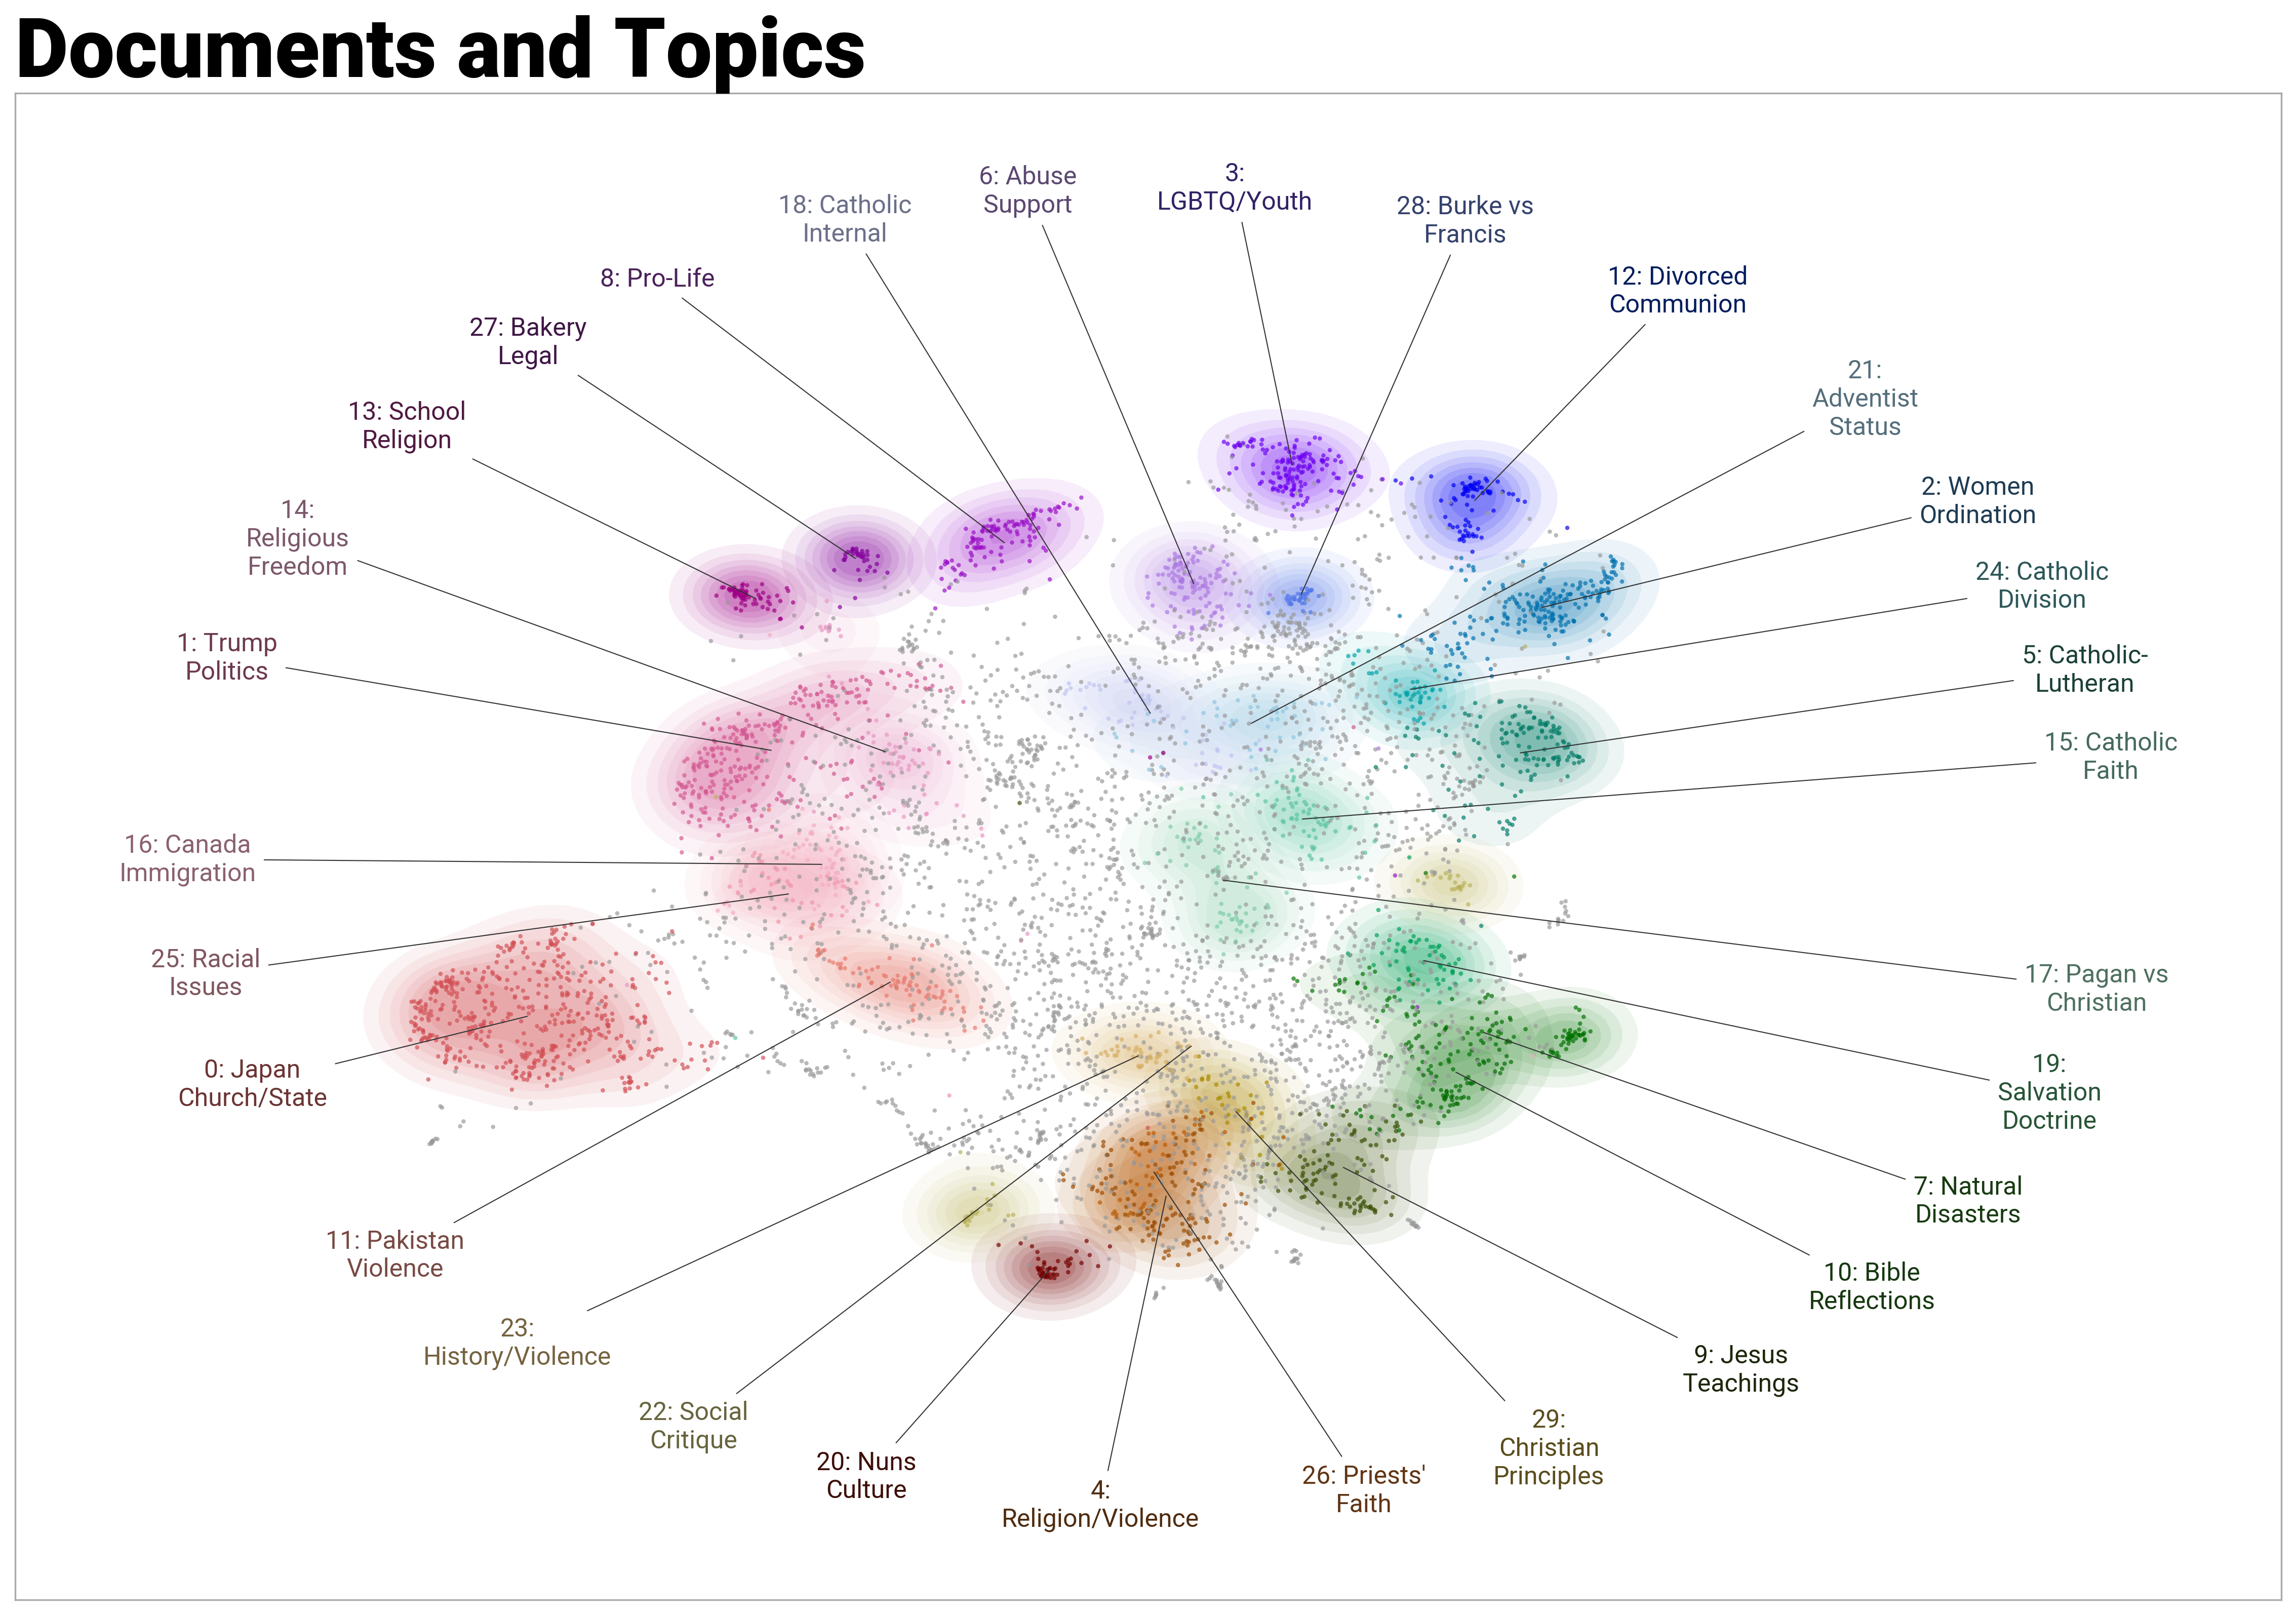
\includegraphics[width=0.68\textwidth]{datamap_final_final.png}\\[0.2em]
  \footnotesize 47 topics, coloured by dominant language.
  \vspace{0.3em}
  \begin{columns}[T,onlytextwidth]
    \begin{column}{0.5\textwidth}\footnotesize
      \textbf{Monolingual peaks.}
      \begin{itemize}
        \item \keyword{JA (99\%)} — Unification Church \& Abe
        \item \keyword{EN (92\%)} — religion \& Canadian identity
        \item \keyword{ZH (96\%)} — missionaries in China
      \end{itemize}
    \end{column}
    \begin{column}{0.5\textwidth}\footnotesize
      \textbf{Truly cross-lingual clusters.} ($H \approx 1.1$)
      \begin{itemize}
        \item LGBTQ+ \& Catholic teaching
        \item Science vs.\ creationism
        \item Conservative / liberal church split
      \end{itemize}
    \end{column}
  \end{columns}
  \vspace{0.3em}
  \takeaway{The corpus is already speaking: some religious grievances are
  local, others travel across languages.}
\end{frame}

% =========================================================================
% FINDING 1 — STABLE TARGET–FRAME RULE
% =========================================================================
\begin{frame}[plain]
  \centering
  \vspace{1.5cm}
  {\Large \textcolor{uzhblue}{\textbf{Finding 1}}}\\[0.4em]
  {\LARGE The target chooses the frame.}\\[0.8em]
  \small \textit{Online religious hostility follows \emph{reusable}
  narrative templates\\ that cross language boundaries.}
\end{frame}

% ---- Slide 7.1: Who is targeted? -----------------------------------------
\begin{frame}{RQ1 — Who is targeted?}
  \begin{columns}[T,onlytextwidth]
    \begin{column}{0.60\textwidth}
      \centering
      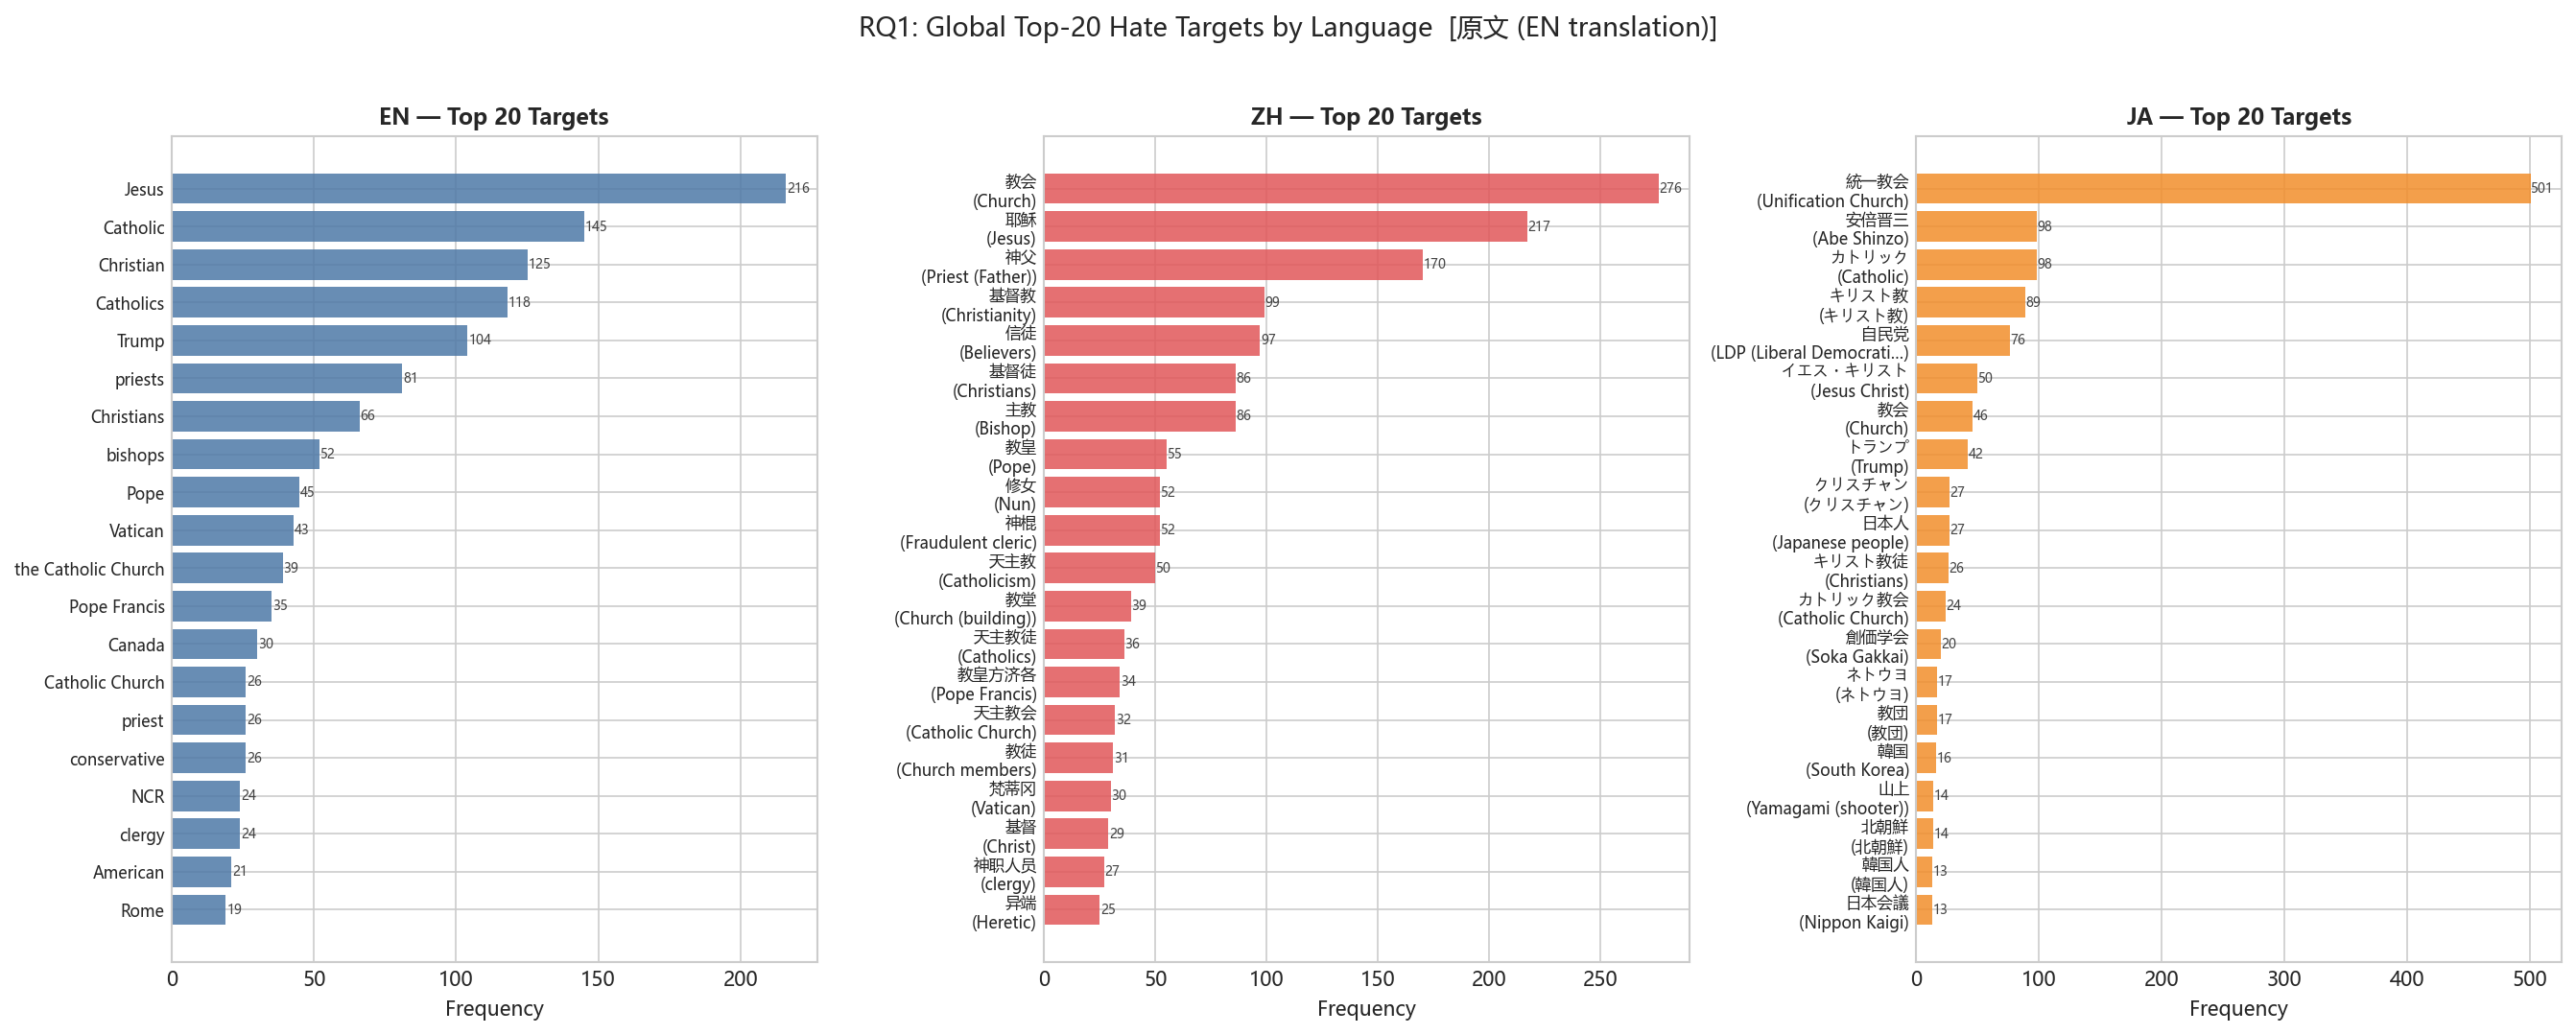
\includegraphics[width=\linewidth]{rq1_global_top20_bilingual.png}
    \end{column}
    \begin{column}{0.39\textwidth}\small
      \textbf{Three distinct target profiles.}
      \begin{itemize}
        \item \keyword{English} — \emph{clergy} dominate; named political
          figures prominent (\textit{priests, bishops, Trump}).
        \item \keyword{Chinese} — \emph{church institutions} and the
          clerical hierarchy; plus 神棍 ``religious fraudster'' — a
          register not seen in the other two languages.
        \item \keyword{Japanese} — \emph{統一教会} (Unification Church)
          alone $= 501$ mentions, dwarfing every other target; paired
          with 安倍晋三 and 自民党.
      \end{itemize}
      \vspace{0.3em}
      \footnotesize
      Japanese hate speech about religion is, in its most prevalent form,
      a discourse about \emphc{domestic political corruption}, not
      theology.
    \end{column}
  \end{columns}
\end{frame}

% ---- Slide 7.2: How is the attack expressed? ------------------------------
\begin{frame}{RQ2 — Which rhetorical frame carries the attack?}
  \small
  \textit{Ten author-constructed frames, induced from pilot-coding 200
  documents and grounded in the framing literature:}
  \vspace{0.4em}
  \begin{columns}[T,onlytextwidth]
    \begin{column}{0.52\textwidth}\footnotesize
      \begin{itemize}
        \item \textbf{Rhetorical Attack} — sarcasm, mockery, invective.
        \item \textbf{Moral Accusation} — hypocrisy, double standards.
        \item \textbf{Sexual Abuse Frame} — clerical abuse \& cover-ups.
        \item \textbf{Economic Exploitation} — fraud, coerced donations.
        \item \textbf{Political Interference} — capture of state / party.
      \end{itemize}
    \end{column}
    \begin{column}{0.48\textwidth}\footnotesize
      \begin{itemize}
        \item \textbf{Cognitive Manipulation} — brainwashing, cult control.
        \item \textbf{Institutional Rot} — systemic cover-up.
        \item \textbf{Social Exclusion} — calls for banning / ostracism.
        \item \textbf{Dehumanization} — vermin / disease metaphors.
        \item \textbf{Other} — residual.
      \end{itemize}
    \end{column}
  \end{columns}
  \vspace{0.2em}
  \centering
  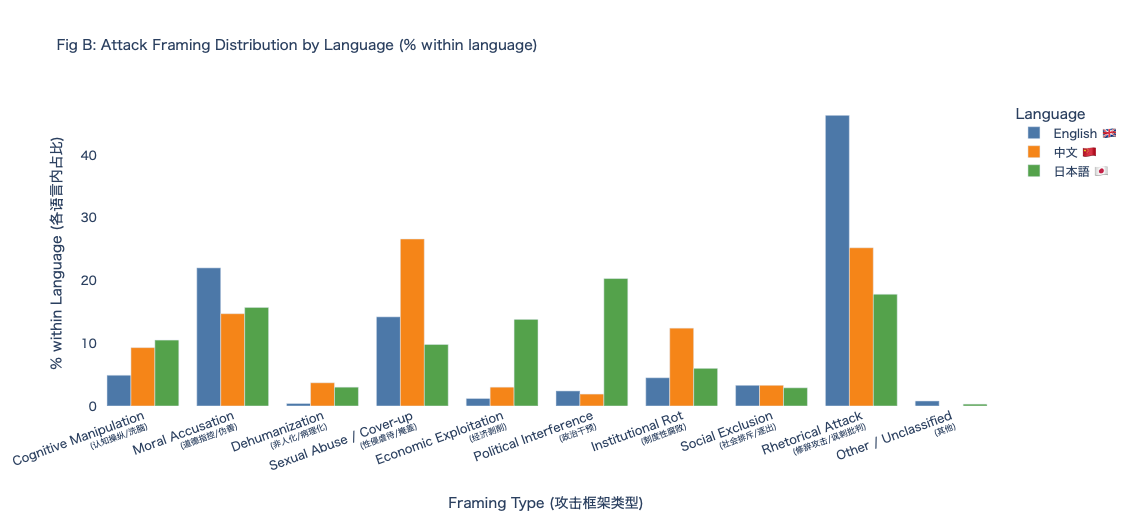
\includegraphics[width=0.78\textwidth]{rq2_lang_tactic.png}
\end{frame}

% ---- Slide 7.2b: Which frames dominate per language -----------------------
\begin{frame}{Three national ``frame signatures''}
  \small
  \begin{columns}[T,onlytextwidth]
    \begin{column}{0.33\textwidth}
      \textbf{\keyword{English}}\\ \footnotesize
      \begin{itemize}
        \item Rhetorical Attack \emph{46\%}
        \item Moral Accusation \emph{22\%}
        \item Sexual Abuse \emph{14\%}
      \end{itemize}
      \footnotesize\textcolor{mutedgray}{``The phony, fake, stifling
      forced artificial piety.'' — broad moral condemnation.}
    \end{column}
    \begin{column}{0.33\textwidth}
      \textbf{\keyword{Japanese}}\\ \footnotesize
      \begin{itemize}
        \item Political Interference \emph{20\%}
        \item Rhetorical Attack \emph{18\%}
        \item Economic Exploitation \emph{14\%}
      \end{itemize}
      \footnotesize\textcolor{mutedgray}{Driven by Abe / 統一教会:
      支配, 献金, 搾取 — politics and money.}
    \end{column}
    \begin{column}{0.33\textwidth}
      \textbf{\keyword{Chinese}}\\ \footnotesize
      \begin{itemize}
        \item Sexual Abuse \emph{26\%}
        \item Rhetorical Attack \emph{25\%}
        \item Moral Accusation \emph{14\%}
      \end{itemize}
      \footnotesize\textcolor{mutedgray}{性侵, 丑闻, 官官相护 —
      clerical misconduct + cover-up.}
    \end{column}
  \end{columns}
  \vspace{0.5em}
  \takeaway{Surface vocabularies differ; but — as the next slide shows —
  the \emph{same underlying rule} chooses them.}
\end{frame}

% ---- Slide 7.3: Target-frame rule (the strongest slide) -------------------
\begin{frame}{The stable target--frame rule}
  \centering
  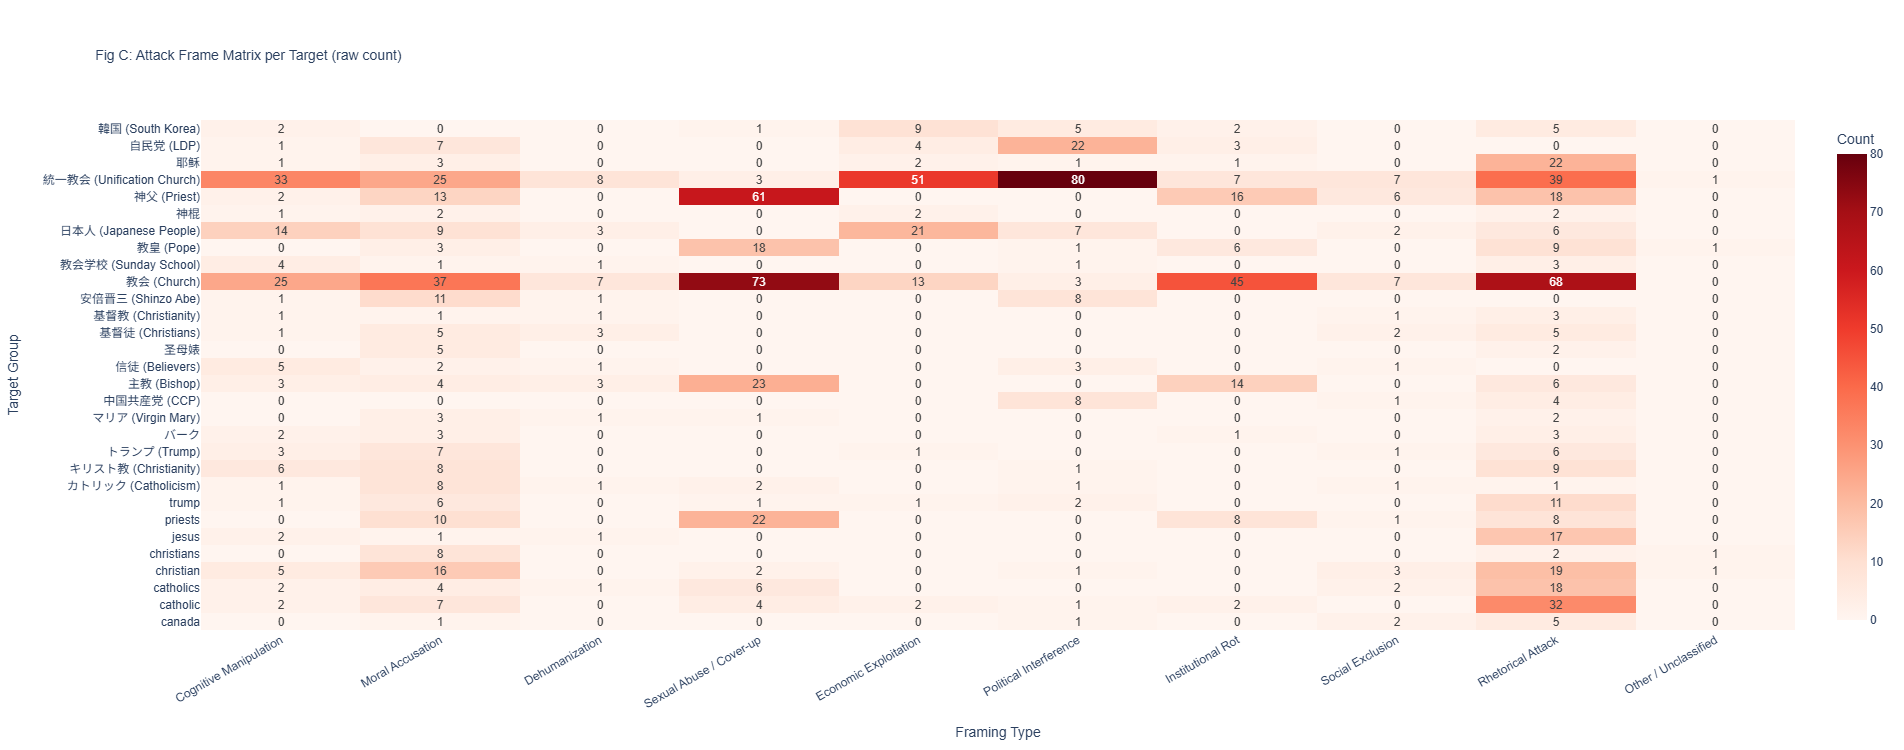
\includegraphics[width=0.64\textwidth]{rq2_target_tactic.png}\\[0.3em]
  \small\textit{Across \emphc{all three languages} — not just within one —
  the target category selects the frame:}
  \vspace{0.3em}
  \begin{center}\small
  \begin{tabular}{@{}r c l@{}}
    \textbf{Clergy} (priests, bishops, Pope)
      & $\longrightarrow$ & \keyword{Sexual Abuse Frame} \\
    \textbf{Institutions} (Unification Church, LDP, 教会)
      & $\longrightarrow$ & \keyword{Political Interference / Economic Exploitation} \\
    \textbf{Collective believers} (Catholics, 基督徒, キリスト教徒)
      & $\longrightarrow$ & \keyword{Rhetorical Attack / Moral Accusation} \\
  \end{tabular}
  \end{center}
  \vspace{0.4em}
  \takeaway{Online hostility against religion behaves like a \emph{genre}
  system: each social category of target activates a recognisable
  narrative template — \keyword{universal in form, localised in vocabulary}.}
\end{frame}

% =========================================================================
% FINDING 2 — DIFFERENT MORAL ARCHITECTURES
% =========================================================================
\begin{frame}[plain]
  \centering
  \vspace{1.5cm}
  {\Large \textcolor{uzhblue}{\textbf{Finding 2}}}\\[0.4em]
  {\LARGE Two moral architectures,\\ one shared target.}\\[0.8em]
  \small \textit{English speakers attack Christianity as a
  \emphc{moral violator}.\\ Chinese and Japanese speakers attack it as a
  \emphc{threat to us}.}
\end{frame}

% ---- Slide 8.1: How to read the RQ3 figure --------------------------------
\begin{frame}{How to read the moral profile}
  \small
  \begin{columns}[T,onlytextwidth]
    \begin{column}{0.52\textwidth}
      Each axis pairs a \emph{virtue} pole with a \emph{vice/threat} pole:
      \vspace{0.2em}
      \begin{itemize}\footnotesize
        \item \textbf{Harm} — care vs.\ harm
        \item \textbf{Fairness} — fairness vs.\ cheating
        \item \textbf{Loyalty} — loyalty vs.\ betrayal
        \item \textbf{Authority} — authority vs.\ subversion
        \item \textbf{Sanctity} — purity vs.\ degradation
        \item \textbf{Realistic Threat} — safety vs.\ invasion
        \item \textbf{Symbolic Threat} — cultural cohesion vs.\ cultural threat
      \end{itemize}
      \vspace{0.2em}
      The score is a cosine similarity between the document and the
      axis vector — it tells us \emph{which moral vocabulary the document
      activates}, not whether the speaker is a fan of the axis.
    \end{column}
    \begin{column}{0.46\textwidth}\footnotesize
      \textbf{Two hostile grammars both show up:}
      \vspace{0.3em}
      \begin{block}{Direct condemnation}
      Vice words fall directly on the target.\\
      \emph{``Christianity is corrupt, harmful, unjust.''}\\
      $\Rightarrow$ \textbf{negative} MFT axes.
      \end{block}
      \begin{block}{Identity defense}
      Ingroup virtue words defend ``us''; target cast as threat.\\
      \emph{``We must protect our sacred tradition from this foreign cult.''}\\
      $\Rightarrow$ \textbf{positive} MFT + \textbf{negative} threat.
      \end{block}
    \end{column}
  \end{columns}
\end{frame}

% ---- Slide 8.2: The main picture -----------------------------------------
\begin{frame}{Three moral fingerprints}
  \centering
  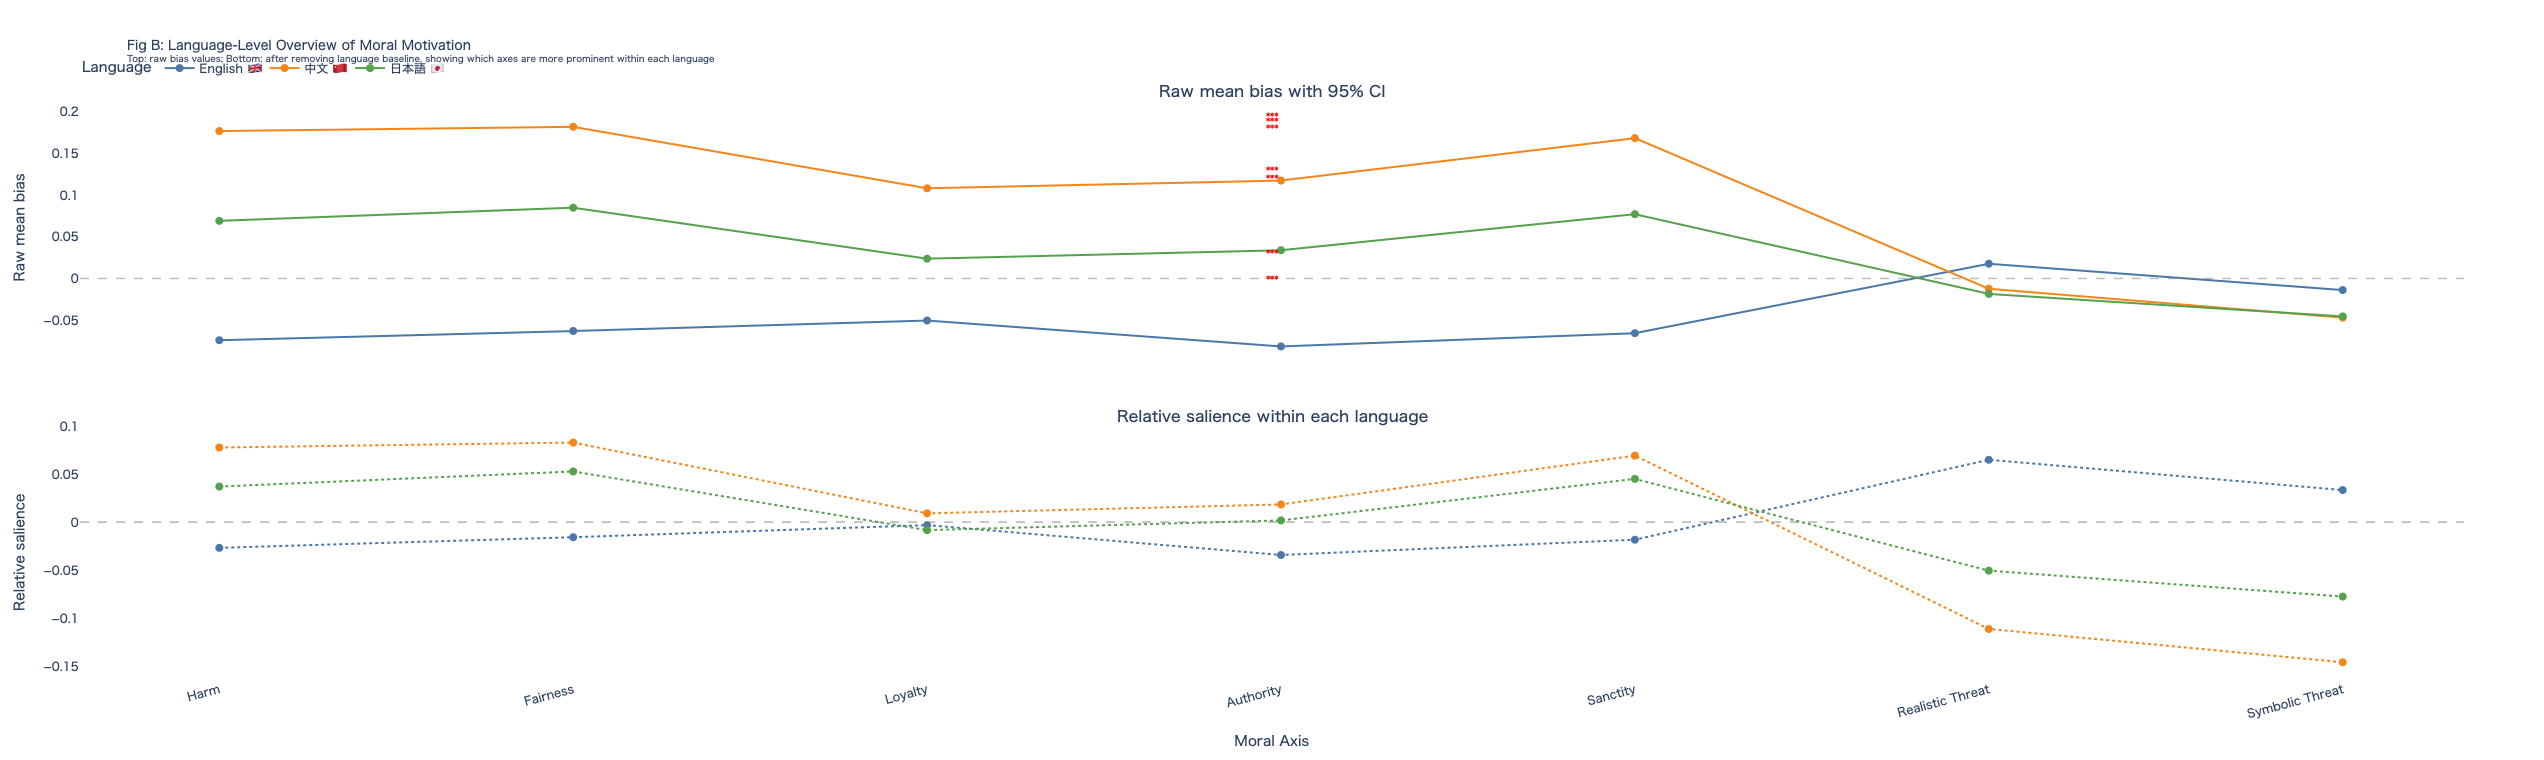
\includegraphics[width=0.80\textwidth]{rq3_lang_line.png}
  \vspace{0.2em}
  \begin{columns}[T,onlytextwidth]
    \begin{column}{0.48\textwidth}\footnotesize
      \textbf{\keyword{English} — direct condemnation.}\\
      Negative on \emph{all five} classical moral foundations.
      Christianity is indicted as ``harmful, unfair, corrupt, authoritarian''
      — a \emphc{wide ethical indictment} from within a shared normative
      framework (insider critique).
    \end{column}
    \begin{column}{0.48\textwidth}\footnotesize
      \textbf{\keyword{Chinese \& Japanese} — identity defense.}\\
      \emph{Positive} on the classical MFT axes; \emph{negative} on
      Symbolic and Realistic Threat. Christianity is framed as a
      \emphc{foreign / social danger} — outsider critique organised
      around group safety.
    \end{column}
  \end{columns}
\end{frame}

% ---- Slide 8.3: Summary ---------------------------------------------------
\begin{frame}{The headline, in one sentence}
  \vspace{0.3em}
  \begin{center}
  \Large
  \textcolor{uzhblue}{\textbf{``Christianity is morally wrong''}}
  \hspace{0.8em}\textit{vs.}\hspace{0.8em}
  \textcolor{uzhaccent}{\textbf{``Christianity is dangerous to us.''}}
  \end{center}
  \vspace{0.6em}
  \small
  \begin{itemize}
    \item Neither grammar is inherently more hostile than the other —
      they are \emph{different rhetorical routes to the same end}.
    \item The choice is not random. It reflects each community's broader
      sense of what \emph{a good society} should look like.
    \item \textit{For Digital-Religion scholars:} the same target
      (Christianity) becomes an analytic lens onto the \emphc{moral
      imaginaries} of three online publics.
  \end{itemize}
\end{frame}

% =========================================================================
% CLOSING
% =========================================================================

% ---- Slide 9: Why this matters beyond anti-Christian speech --------------
\begin{frame}{What the framework offers beyond this case}
  \small
  The \emph{who--how--why} pipeline is \keyword{target-agnostic}.
  The same three-stage design can be pointed at:
  \vspace{0.3em}
  \begin{columns}[T,onlytextwidth]
    \begin{column}{0.48\textwidth}
    \begin{itemize}
      \item Islamophobia across Europe and South Asia
      \item Antisemitic rhetoric on Telegram, YouTube
      \item Anti-Hindu discourse in South-Asian diasporas
    \end{itemize}
    \end{column}
    \begin{column}{0.48\textwidth}
    \begin{itemize}
      \item Sectarian conflict (Sunni / Shi`a; Catholic / Protestant)
      \item Religion \& nationalism studies
      \item Minority / majority reversals across regions
    \end{itemize}
    \end{column}
  \end{columns}
  \vspace{0.4em}
  \takeaway{The contribution is a \keyword{framework}, not only a
  Christianity case-study — a reusable way for religion scholars to
  interrogate large-scale digital discourse at interpretable
  resolution.}
\end{frame}

% ---- Slide 10: Limits + invitation ---------------------------------------
\begin{frame}{Limits, and what I want to discuss with you}
  \small
  \textbf{Honest limits.}
  \begin{itemize}
    \item \emph{Platform bias.} Tieba, 5ch, and Anglophone forums each
      carry their own selection effects.
    \item \emph{Constructed datasets.} Our annotated Chinese / Japanese
      data are partly back-translation-augmented.
    \item \emph{Moral dictionaries} were built for English; the CMFD /
      J-MFD adaptations are imperfect.
    \item \emph{Qualitative validation} by religion scholars is still
      needed topic-by-topic — this is where \textbf{you} come in.
  \end{itemize}
  \vspace{0.4em}
  \textbf{Three discussion questions.}
  \begin{enumerate}\small
    \item How should Digital-Religion studies draw the line between
      \emph{hostility} and \emph{critique}?
    \item Can computational models be trained to detect
      \emph{theological} nuance — not only discursive hostility?
    \item Which traditions should be compared next? Where would the
      \emph{who--how--why} framework break?
  \end{enumerate}
\end{frame}

% ---- Slide 11: Thank you --------------------------------------------------
\begin{frame}[plain]
  \vspace{1.5cm}
  \centering
  {\Large\textcolor{uzhblue}{\textbf{Thank you.}}}\\[0.8em]
  {\small From binary detection\\
  toward \emphc{structured, cross-cultural interpretation}\\
  of religious discourse online.}\\[1.2em]
  \small
  \textbf{Zhidian Huang}\\
  huangzhidian15@gmail.com\\
  \href{https://github.com/notsofun/Master_Thesis}{github.com/notsofun/Master\_Thesis}
  \vspace{0.8em}\\
  \footnotesize\textit{I'd love your questions — especially the hard ones.}
\end{frame}

\end{document}
notsofun/Master_Thesis}{github.com/notsofun/Master\_Thesis}
  \vspace{0.8em}\\
  \footnotesize\textit{I'd love your questions — especially the hard ones.}
\end{frame}

\end{document}
ster_Thesis}{github.com/notsofun/Master\_Thesis}
  \vspace{0.8em}\\
  \footnotesize\textit{I'd love your questions — especially the hard ones.}
\end{frame}

\end{document}
